% Compile with: xelatex main.tex (run twice for TOC/references)
% Or use latexmk: latexmk -xelatex main.tex

\documentclass[12pt,a4paper]{report}

% University of Pécs FTIK — diploma thesis layout
\usepackage[a4paper, top=4cm, bottom=2.5cm, right=2.5cm, left=3.5cm]{geometry}
\usepackage{setspace}
\onehalfspacing
\usepackage{parskip}
\usepackage{ragged2e}
\justifying

\usepackage{fontspec}
\setmainfont{Times New Roman}
\setsansfont{Arial}

\usepackage{titlesec}
\titleformat{\chapter}[display]{\sffamily\bfseries\fontsize{14}{16}\selectfont}{\chaptertitlename\ \thechapter}{1em}{}
\titlespacing*{\chapter}{0pt}{0pt}{1.5em}
\titleformat{\section}{\sffamily\bfseries\fontsize{12}{14}\selectfont}{\thesection}{1em}{}
\titleformat{\subsection}{\sffamily\bfseries\fontsize{12}{14}\selectfont}{\thesubsection}{1em}{}
\titlespacing*{\section}{0pt}{1em}{1em}
\titlespacing*{\subsection}{0pt}{1em}{1em}

\usepackage{graphicx}
\usepackage{booktabs}
\usepackage{longtable}
\usepackage{amsmath}
\usepackage{enumitem}
\usepackage{caption}
\captionsetup{font=small, labelfont=bf}
\usepackage{fancyhdr}
\pagestyle{fancy}
\fancyhf{}
\fancyfoot[C]{\thepage}
\renewcommand{\headrulewidth}{0pt}
\fancyhead[C]{\small\textit{Secure Cloud-Based Healthcare Appointment Management System (DocBook)}}

\usepackage{hyperref}
\hypersetup{colorlinks=true, linkcolor=black, citecolor=black, urlcolor=blue}

\setcounter{secnumdepth}{3}
\setcounter{tocdepth}{3}

\newcommand{\thesistitle}{Secure Cloud-Based Healthcare Appointment Management System (DocBook)}
\newcommand{\thesisauthor}{Abdulkadir Salihu Abdulhamid}
\newcommand{\thesissupervisor}{[SUPERVISOR\_NAME]}
\newcommand{\thesisnumber}{[THESIS\_NUMBER]}
\newcommand{\thesisyear}{2026}


\usepackage[style=numeric,sorting=none]{biblatex}
\addbibresource{references.bib}

\begin{document}

\begin{titlepage}
  \centering
  \vspace*{2cm}
  {\large Number: \thesisnumber/2026\par}
  \vspace{2cm}
  {\Large\bfseries DIPLOMA WORK\par}
  \vspace{1.5cm}
  {\LARGE\bfseries \thesistitle\par}
  \vspace{2cm}
  {\large Author: \thesisauthor\par}
  \vspace{0.5cm}
  {\large Year: \thesisyear\par}
  \vfill
  University of Pécs\\
  Faculty of Engineering and Information Technology\\
  Computer Science Engineering Bachelor
\end{titlepage}

\newpage
\thispagestyle{empty}
\begin{center}
  {\Large\bfseries DIPLOMA WORK\par}
  \vspace{1cm}
  {\LARGE\bfseries \thesistitle\par}
  \vspace{2cm}
  Author: \thesisauthor\\
  Supervisor: \thesissupervisor\\
  \vfill
  Pécs, \thesisyear
\end{center}

\newpage
\chapter*{Declaration}
I declare that this diploma thesis is the result of my own work. All references and external works have been identified and cited. I have not used any other external help.

The results of my diploma work can be used by the university for its own purposes free of charge.

\vspace{2cm}
Pécs, [SUBMISSION\_DATE]

\hfill ................................................\\
\hfill Signature of the student

\tableofcontents
\newpage


\chapter{Introduction}

Healthcare organisations depend on reliable scheduling so that patients receive care on time and clinical staff can plan their work efficiently. In many clinics and hospitals, appointments are still arranged by telephone, paper registers, or informal messaging. These methods are slow, error-prone, and difficult to audit. When several receptionists maintain separate notebooks, double booking and lost records become frequent. Patients who cannot reach the clinic by phone may delay treatment. Doctors lack a single view of the day's consultations. Administrators cannot easily measure utilisation or revenue. A dedicated web application that runs in the cloud can centralise appointment data, enforce security rules, and give each stakeholder---patient, doctor, and administrator---a clear interface for their tasks.

The global shift toward digital health accelerated after widespread adoption of internet services and mobile devices. The World Health Organization promotes digital health as a means to strengthen health systems and improve outcomes~\cite{who2024}. For computer science engineering, an appointment system is an appropriate diploma topic because it combines databases, human--computer interaction, security engineering, and distributed deployment in one coherent product.

The aim of this diploma work is to design, implement, test, and deploy \textbf{DocBook}, a secure cloud-based healthcare appointment management system. The name \textbf{DocBook} reflects the purpose: a digital record of doctor appointments and related administrative data. The personal motivation for this topic came from observing how outpatient clinics struggle with manual scheduling during peak hours. I wanted to build a system that could be demonstrated to examiners both locally and through a stable HTTPS URL.

\section{Objectives}

The approved diploma tasks define the following primary objectives:

\begin{enumerate}
  \item Analyse the requirements of a secure, web-based healthcare appointment system for patients, doctors, and administrators.
  \item Design and implement a role-based application that supports appointment scheduling, tracking, and management.
  \item Implement secure authentication with encrypted password storage and access control for each user role.
  \item Deploy the system to a cloud platform with HTTPS protection and document the architecture, tests, and results.
\end{enumerate}

\textbf{Scope included:} user registration and login, doctor search, slot-based booking, dashboards, prescriptions with rich text, admin CRUD for specialities, appointment and revenue reports, automated demo data for evaluation.

\textbf{Scope excluded:} payment gateways, insurance billing, video telemedicine, native mobile applications, and integration with national electronic health record systems.

The core problem is to provide a single web platform where patients can discover doctors and book appointments; doctors can publish schedules and manage visits; administrators can monitor the institution. The system must prevent users from accessing functions outside their role. Login credentials must never be stored in plain text. In production, all communication must use HTTPS.

\chapter{Literature Review}

\section{Overview of Healthcare Appointment Systems}

Healthcare appointment scheduling sits at the intersection of medicine, information technology, and service operations. Clinics must match finite doctor time with patient demand while minimising no-shows and idle capacity. Before computerisation, paper diaries and wall calendars performed this function. Computerised systems introduced searchable records, automated reminders, and statistical reports. Web-based systems further removed the need for patients to visit the clinic physically to reserve a slot. Cloud hosting removed the need for each clinic to maintain its own server room.

Digital health services have expanded rapidly. Patients expect to book consultations online, and providers need systems that respect privacy and role separation. For a computer science engineering project, it is essential to demonstrate not only user-facing features but also secure engineering practice: correct authentication, authorisation, and deployment on infrastructure that supports TLS encryption.

During my studies I identified a gap between simple demonstration websites and production-oriented applications. I therefore set out to build a complete system that could be demonstrated locally and also deployed on a public cloud URL with a real database, which is closer to industry practice than a prototype that runs only on a developer laptop.

\section{Theoretical Framework}

Healthcare appointment systems should be designed around the needs of real users rather than around database tables alone. User-Centered Design (UCD) provides a suitable theoretical basis for this thesis.

\subsection{User-Centered Design (UCD) Principles}

User-centered design is an iterative process that focuses on users and their needs at every stage of development. It emphasises understanding the target audience through research and design techniques so that the product is usable, accessible, and aligned with real tasks. The figure below shows the iterative principles of UCD (Figure~\ref{fig:ucd}).

\begin{figure}[htbp]
  \centering
  \includegraphics[width=0.95\textwidth]{figures/ucd-principles}
  \caption{UCD principles}
  \label{fig:ucd}
\end{figure}

In the context of \textbf{DocBook}, I did not run a full formal user-study programme with clinicians and patients at every iteration, but I applied UCD principles in a structured, intuitive way: I analysed how patients, doctors, and administrators work when appointments are booked manually, and I translated those needs into screens and workflows. For \textbf{patients}, the focus was on simple search, clear available slots, and visible appointment status. For \textbf{doctors}, the focus was on setting weekly availability, confirming bookings quickly, and recording prescriptions after a visit. For \textbf{administrators}, the focus was on overview dashboards and reports without exposing clinical tools meant for doctors.

This approach addressed typical problems in healthcare scheduling: long phone queues, unclear availability, double booking, and lack of a single view of the day's appointments. As noted in usability literature, understanding user needs and reflecting them in the interface is essential for adoption and correct use of digital health tools~\cite{iso9241}. DocBook was designed so that each role sees only relevant functions, which supports both usability and security.

\subsection{Core Features Guided by UCD Principles}

\begin{table}[htbp]
  \centering
  \caption{UCD principles mapped to DocBook features}
  \label{tab:ucd-features}
  \begin{tabular}{@{}p{4.5cm}p{8cm}@{}}
    \toprule
    UCD principle & DocBook feature \\
    \midrule
    Visibility of status & Appointment states: pending, confirmed, completed \\
    Error prevention & Unique constraint prevents double booking \\
    Recognition over recall & Dashboard lists upcoming appointments \\
    Role-appropriate UI & Separate patient, doctor, admin interfaces \\
    Trust and security & HTTPS, hashed passwords, RBAC \\
    \bottomrule
  \end{tabular}
\end{table}

\section{Comparative Analysis of Existing Systems}

\subsection{Healthcare and Appointment Platforms}

Commercial hospital systems integrate scheduling with billing and clinical records. They are powerful but expensive. Consumer booking platforms focus on discovery and booking for private practice. DocBook positions itself as an educational full-stack implementation with documented security and open deployability, not as a commercial competitor.

\begin{table}[htbp]
  \centering
  \caption{Comparison of approach types}
  \label{tab:approach-types}
  \begin{tabular}{@{}p{2.2cm}p{3.2cm}p{3.2cm}p{4.5cm}@{}}
    \toprule
    Type & Strength & Limitation & DocBook response \\
    \midrule
    Paper diary & Simple & No remote access & Web database \\
    Spreadsheet & Flexible & No RBAC & Multi-user app with roles \\
    Full HIS & Complete & High cost & Focused appointment module \\
    Generic demo & Fast build & No workflow & Full appointment lifecycle \\
    \bottomrule
  \end{tabular}
\end{table}

\subsection{Identified Gaps and Solutions}

\begin{table}[htbp]
  \centering
  \caption{Identified gaps and DocBook solutions}
  \label{tab:gaps}
  \begin{tabular}{@{}p{5.5cm}p{7cm}@{}}
    \toprule
    Gap & Solution \\
    \midrule
    No role separation & RBAC mixins per role \\
    Weak passwords & PBKDF2-SHA256 hashing \\
    No cloud HTTPS demo & Render deployment with TLS \\
    Double booking & Database uniqueness constraint \\
    No admin reporting & Appointment and revenue reports \\
    \bottomrule
  \end{tabular}
\end{table}

\chapter{Specification and Solution Approach}

\section{Specification}
\label{sec:specification}

The requirements for \textbf{DocBook} were derived from studying how outpatient clinics operate in practice. A patient contacts the clinic; staff check the doctor's diary (paper or spreadsheet), reserve a slot, and later mark the visit as completed or missed. When several people work without one shared system, the same slot can be promised twice, data can be entered incorrectly, and there is no clear record of who changed an appointment.

Translating this process into software requires \textbf{data validation} (correct dates, required fields, consistent status values), \textbf{concurrency} (only one patient may book a given doctor at a given date and time), and \textbf{accountability} (status changes are tied to the logged-in role). DocBook must also support patients, doctors, and administrators through \textbf{role-based access control} and basic security (hashed passwords, CSRF protection, HTTPS in production). The subsections below list functional and non-functional requirements, stakeholder needs, the manual workflow, use cases, and risks---against which Chapters 4--6 were developed.

\subsection{Functional requirements}

\begin{table}[htbp]
  \centering
  \caption{Functional requirements}
  \begin{tabular}{@{}cl@{}}
    \toprule
    ID & Requirement \\
    \midrule
    FR-1 & Public pages (home, terms, privacy) and doctor listing with search \\
    FR-2 & Patients register, log in, book, view and cancel bookings, add reviews \\
    FR-3 & Doctors set schedules, accept or reject appointments, manage patients, prescriptions \\
    FR-4 & Administrators access dashboard with user, appointment, speciality, and reports \\
    FR-5 & Prevent double booking of the same doctor at the same date and time \\
    FR-6 & Appointment status: pending, confirmed, completed, cancelled, no\_show \\
    \bottomrule
  \end{tabular}
\end{table}

\subsection{Non-functional requirements}

\begin{table}[htbp]
  \centering
  \caption{Non-functional requirements}
  \begin{tabular}{@{}cl@{}}
    \toprule
    ID & Requirement \\
    \midrule
    NFR-1 & Passwords stored using one-way hash (PBKDF2-SHA256) \\
    NFR-2 & Forms protected against CSRF \\
    NFR-3 & Production enforces HTTPS, secure cookies, and HSTS \\
    NFR-4 & Application runs on Python 3.12 and Django 5.0.6 \\
    NFR-5 & Configuration secrets loaded from environment variables \\
    NFR-6 & Static assets served efficiently in production (WhiteNoise) \\
    \bottomrule
  \end{tabular}
\end{table}

\subsection{Stakeholder analysis}

\begin{itemize}
  \item \textbf{Patients} need simplicity, clear availability, and trust in data handling.
  \item \textbf{Doctors} need accurate schedules and quick status updates on appointments.
  \item \textbf{Administrators} need overview statistics and control over specialities and content.
  \item \textbf{Developers / maintainers} need modular Django apps and documented deployment steps.
\end{itemize}

\subsection{Analysis of the current situation (manual process)}

Before automation, a typical small clinic workflow can be described in five steps: (1) the patient calls or visits reception; (2) staff look up the doctor's paper diary; (3) a slot is verbally agreed; (4) the name is written in the diary; (5) on the day of visit the doctor marks attendance informally. This process has weaknesses. Paper diaries are not searchable by specialisation across many doctors. Changes require physical access to the book. There is no automatic reminder. Reporting on monthly appointments or revenue requires manual counting.

DocBook digitises steps 1--5. Search replaces browsing paper lists. The database replaces the diary. Status fields replace marginal notes. Reports query the database directly. The analysis shows that the highest value is not fancy graphics but \textbf{correct data model, access control, and reliable hosting}.

\subsection{Use cases}

\subsubsection{Patient books an appointment}

\textbf{Actor:} registered patient. \textbf{Precondition:} doctor has published schedule slots. \textbf{Main flow:} patient logs in, searches for doctor, opens profile, selects date and time, submits booking, receives confirmation with pending status. \textbf{Alternative flow:} slot already taken---system shows error and offers another slot. \textbf{Postcondition:} booking record exists with status pending.

\subsubsection{Doctor confirms appointment}

\textbf{Actor:} registered doctor. \textbf{Precondition:} pending booking exists for that doctor. \textbf{Main flow:} doctor opens appointment list, selects booking, chooses confirm action. \textbf{Postcondition:} status becomes confirmed; patient sees updated state on dashboard.

\subsubsection{Administrator generates report}

\textbf{Actor:} superuser administrator. \textbf{Precondition:} historical bookings exist. \textbf{Main flow:} admin logs in, navigates to appointment report, filters by period, reads aggregated counts. \textbf{Postcondition:} no data change; information supports management decisions.

\subsection{Risk analysis}

\begin{table}[htbp]
  \centering
  \caption{Risk analysis and mitigations}
  \begin{tabular}{@{}p{4.5cm}cl@{}}
    \toprule
    Risk & Impact & Mitigation in DocBook \\
    \midrule
    Unauthorised access to medical data & High & RBAC, login required, HTTPS \\
    Password leakage & High & Hashing, no plain-text storage \\
    Double booking & Medium & DB uniqueness constraint \\
    CSRF on forms & Medium & Django CSRF middleware \\
    Downtime on free cloud tier & Low & Acceptable for thesis demo; paid tier for production \\
    Weak demo passwords & Medium & Documented warning; change in real deployment \\
    \bottomrule
  \end{tabular}
\end{table}

\section{Solution Approach}

Given the requirements in Section~\ref{sec:specification}, the chosen solution is a \textbf{Django monolith}: one Python application that handles authentication, business logic, HTML pages, and database access. This approach was preferred over a separate single-page frontend because it reduces deployment complexity, keeps session-based login straightforward, and matches the skills emphasised in the computer science engineering programme. The user interface uses \textbf{server-rendered templates} (Bootstrap, jQuery, HTMX where partial updates help), with \textbf{Django REST Framework} for selected API endpoints such as profile updates.

For development, the project runs locally with \textbf{SQLite}; for the thesis demonstration it is deployed on \textbf{Render.com} with \textbf{PostgreSQL}, \textbf{Gunicorn}, and \textbf{WhiteNoise} for static files. Production settings enforce HTTPS, secure cookies, and secrets from environment variables. The following subsections describe the backend, frontend, and tools---in the same order used in comparable diploma theses.

\subsection{Backend}

The backend uses Python 3.12 and Django 5.0.6 with applications \texttt{accounts}, \texttt{doctors}, \texttt{patients}, \texttt{bookings}, and \texttt{core}. Authentication is session-based. The ORM maps to SQLite locally and PostgreSQL in production. Gunicorn serves WSGI requests; WhiteNoise serves static files.

\subsection{Frontend}

The frontend uses server-rendered Django templates with Bootstrap for layout, jQuery for interactions, HTMX for partial updates, and Chart.js on the admin dashboard. Django REST Framework supports profile API endpoints. This avoids a separate SPA build while remaining responsive enough for the thesis demonstration.

\subsection{Tools and Development Environment}

\begin{table}[htbp]
  \centering
  \caption{Development tools}
  \begin{tabular}{@{}ll@{}}
    \toprule
    Tool & Purpose \\
    \midrule
    Python 3.12.8 & Runtime \\
    Django 5.0.6 & Web framework \\
    Git / GitHub & Version control \\
    Render.com & Cloud hosting \\
    PostgreSQL & Production database \\
    Chrome & Testing and screenshots \\
    \bottomrule
  \end{tabular}
\end{table}

\chapter{System Design and Architecture}

DocBook follows a three-tier architecture: presentation (HTML templates), application (Django views and business logic), and data (SQLite or PostgreSQL). Figure~\ref{fig:architecture} illustrates the production deployment view.

\begin{figure}[htbp]
  \centering
  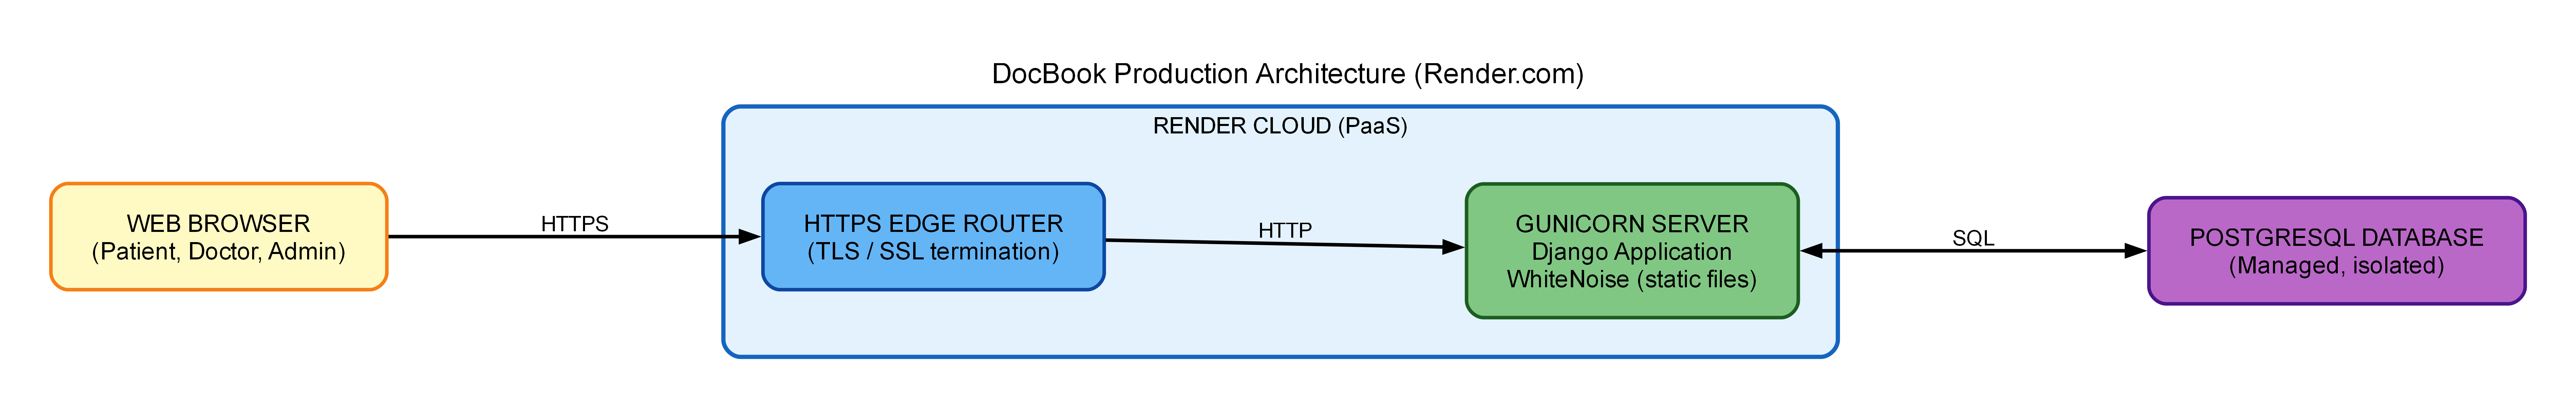
\includegraphics[width=\textwidth]{figures/docbook_architecture}
  \caption{Cloud infrastructure architecture of DocBook on Render: user traffic enters over HTTPS, is terminated at the edge router, processed by Gunicorn and Django (with WhiteNoise for static files), and persists in an isolated PostgreSQL database}
  \label{fig:architecture}
\end{figure}

\section{Database Design}

The central entity is a custom \textbf{User} model with role \texttt{doctor} or \texttt{patient}. A one-to-one \textbf{Profile} stores extended attributes. \textbf{Booking} links doctor and patient with date, time, and status; \texttt{unique\_together} on \texttt{(doctor, appointment\_date, appointment\_time)} prevents double booking. \textbf{Prescription} extends a booking one-to-one. \textbf{Review} links patient, doctor, and booking with a 1--5 rating. Figure~\ref{fig:erd} shows the entity-relationship layout generated from the Django models (\texttt{accounts}, \texttt{bookings}, \texttt{core}).

\begin{figure}[htbp]
  \centering
  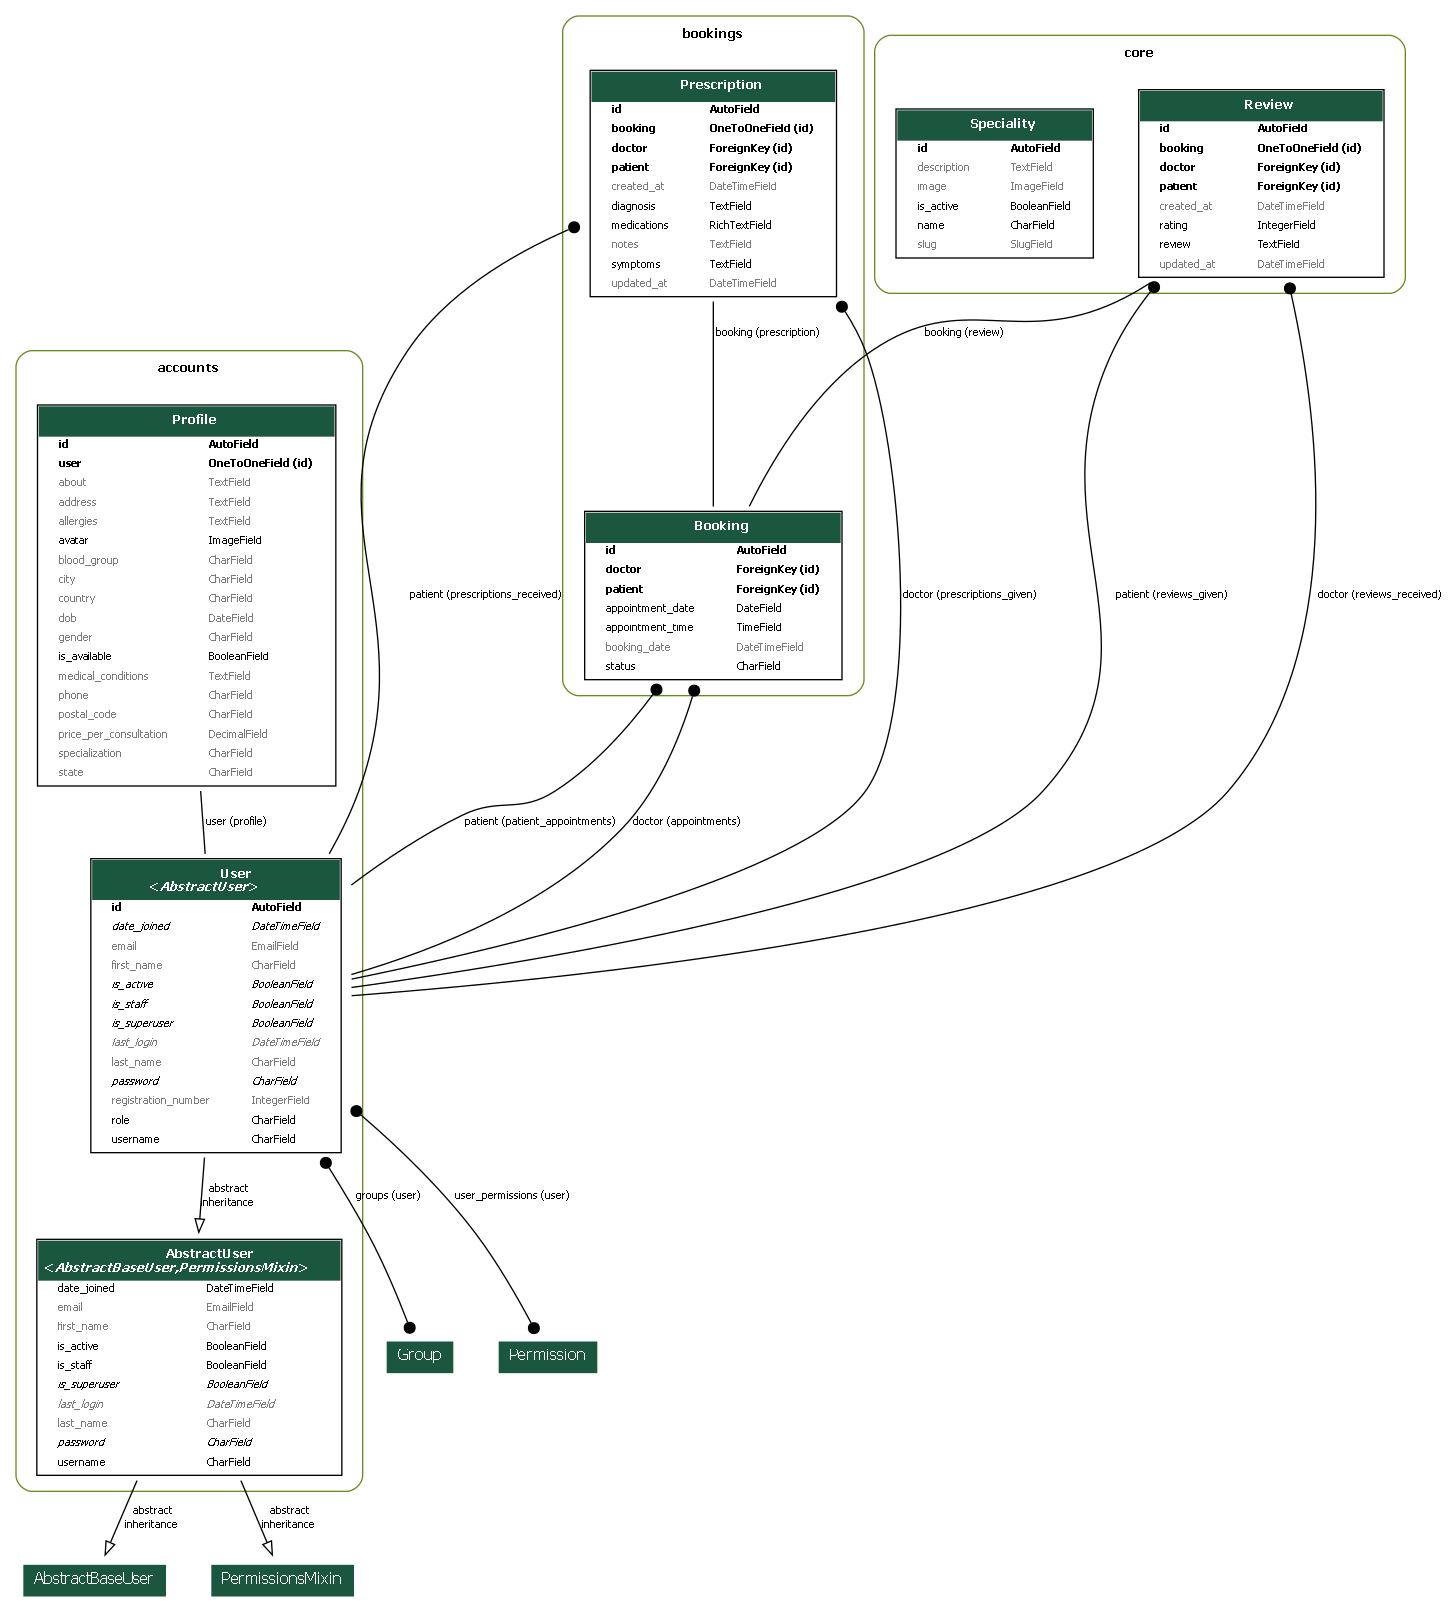
\includegraphics[width=\textwidth]{figures/docbook_erd}
  \caption{Entity-relationship diagram of DocBook core entities}
  \label{fig:erd}
\end{figure}

\section{Backend Design}

Role-based access control uses \texttt{PatientRequiredMixin}, \texttt{DoctorRequiredMixin}, and \texttt{AdminRequiredMixin}. Object-level checks ensure patients access only their own bookings. Middleware includes security, CSRF, session, and authentication layers.

\section{Frontend Design}

\subsection{Django Templates and Bootstrap}
Templates extend a common base layout. Navigation is role-specific after login.

\subsection{HTMX}
Used for partial updates on doctor profile forms without full page reload.

\subsection{jQuery and Chart.js}
jQuery supports legacy components; Chart.js renders admin dashboard statistics.

\subsection{Django REST Framework}
JSON endpoints update profile fragments where asynchronous behaviour helps.

\subsection{URL Routing Structure}
Public routes under \texttt{/}, authentication under \texttt{/accounts/}, role dashboards under \texttt{/patients/}, \texttt{/doctors/}, and \texttt{/admin/}.

\section{Use Case Diagrams}

Actors: Patient, Doctor, Administrator. Main use cases: book appointment, confirm appointment, manage schedule, view reports. (Insert diagram exported from draw.io or Word.)

\section{Wireframes and Interface Screens}

Insert screenshots of home page, login, patient dashboard, doctor schedule, booking confirmation, and admin dashboard as Figures in this section. See Appendix for the full list.

\chapter{Implementation}

\section{Django Stack Development}

\subsection{Backend Setup}

Development used Windows 11, Python 3.12, virtual environment, and Git. Local setup:

\begin{verbatim}
python -m venv venv
pip install -r requirements.txt
python manage.py migrate
python manage.py loaddata fixtures/initial_data.json
python create_admin.py
python manage.py runserver
\end{verbatim}

\subsection{Frontend Setup}

Templates live under \texttt{templates/}; static assets under \texttt{static/}. \texttt{collectstatic} prepares files for production; WhiteNoise serves them on Render.

\section{Configuration Setup}

\subsection{Middleware}

Order: SecurityMiddleware, WhiteNoise, Session, Common, CSRF, Authentication, Messages, XFrameOptions.

\subsection{Routes}

URL configuration in \texttt{docbook/urls.py} includes apps for accounts, patients, doctors, bookings, core, and admin views.

\subsection{Database Models}

Key models: \texttt{User}, \texttt{Profile}, \texttt{Booking}, \texttt{Prescription}, \texttt{Review}, day schedule models, and \texttt{TimeRange}.

\section{Authentication and Authorization}

Login uses Django \texttt{authenticate()} and session cookies. Passwords are hashed with PBKDF2-SHA256. RBAC mixins guard class-based views; decorators guard selected function views.

\section{Appointment Booking Workflow}

\subsection{Schedule and Slot Generation}
Doctors configure weekly availability; the UI derives bookable slots from time ranges minus existing bookings.

\subsection{Booking Creation and Status Management}
Patients create bookings with status \texttt{pending}; doctors confirm, complete, cancel, or mark \texttt{no\_show}.

\subsection{Prescription and Review Processing}
Doctors add prescriptions via CKEditor; patients submit reviews after completed visits.

\section{Administrative Dashboard and Reports}

Custom admin at \texttt{/admin/} provides statistics, user lists, speciality CRUD, and appointment/revenue reports. Django admin remains at \texttt{/super-admin/}.

\section{Cloud Deployment on Render}

Build command: \texttt{bash build.sh}. Start command: \texttt{gunicorn docbook.wsgi:application --bind 0.0.0.0:\$PORT}. Environment variables: \texttt{SECRET\_KEY}, \texttt{DEBUG=False}, \texttt{ALLOWED\_HOSTS}, \texttt{DATABASE\_URL}, \texttt{CSRF\_TRUSTED\_ORIGINS}.

Live URL: \url{https://healthcare-appointment-system-9a2r.onrender.com}

\section{Security and HTTPS Configuration}

When \texttt{DEBUG=False}, settings enable SSL redirect, secure cookies, HSTS, and trusted CSRF origins.

\section{User Interface Implementation}

The public home page supports doctor search; role dashboards show appointments and actions appropriate to each user type.

\chapter{Testing and Feedback}

\section{Test Strategy}

Testing combined Django unit tests, Selenium end-to-end tests, and manual verification on the deployed system.

\section{Functional Testing}

Registration, login, booking, doctor schedule update, admin dashboard, and double-booking prevention were tested. Automated tests run with \texttt{python manage.py test tests}.

\section{Security Testing}

Password fields store \texttt{pbkdf2\_sha256} hashes. CSRF tokens appear on forms. RBAC tests: patient cannot access doctor dashboard (HTTP 403 or redirect). Production uses HTTPS.

\section{Evaluation and Feedback}

All functional and non-functional requirements from Chapter~3 were satisfied. Classmates provided informal feedback on usability of the booking flow. Limitations include minimal password policy and Render free-tier cold starts.

\chapter{Conclusion and Future Development}

\section{Conclusion}

This diploma thesis presented the design, implementation, testing, and deployment of \textbf{DocBook}, a secure cloud-based healthcare appointment management system. The work delivered separate interfaces for patients, doctors, and administrators; RBAC; encrypted authentication; a complete appointment lifecycle; administrative reporting; and cloud deployment with HTTPS.

The project objectives from the task specification were fulfilled. The system is suitable for final examination demonstration and as a foundation for future extensions.

\section{Future Development}

Short-term improvements: password reset email, stronger password policy, login rate limiting. Medium-term: SMS/email reminders, calendar export. Long-term: payment integration, FHIR APIs, two-factor authentication for clinical roles.


\chapter*{References}
\addcontentsline{toc}{chapter}{References}
\printbibliography[heading=none]

\appendix
\chapter{User Manual}
Production URL: \url{https://healthcare-appointment-system-9a2r.onrender.com}. Demo accounts: \texttt{patient1}, \texttt{doctor1}, \texttt{admin} with password \texttt{aaa} (academic use only).

\chapter{Source Code Structure}
Project root: \texttt{secure-cloud-based-healthcare-appointment-system/} with Django apps \texttt{accounts}, \texttt{core}, \texttt{doctors}, \texttt{patients}, \texttt{bookings}.

\chapter{Screenshots and Figures}
Insert all UI screenshots here if not placed in Chapter~4 and~5. Use continuous figure numbering across the thesis.

\end{document}
